%% 
%% Copyright 2007-2025 Elsevier Ltd
%% 
%% This file is part of the 'Elsarticle Bundle'.
%% ---------------------------------------------
%% 
%% It may be distributed under the conditions of the LaTeX Project Public
%% License, either version 1.3 of this license or (at your option) any
%% later version.  The latest version of this license is in
%%    http://www.latex-project.org/lppl.txt
%% and version 1.3 or later is part of all distributions of LaTeX
%% version 1999/12/01 or later.
%% 
%% The list of all files belonging to the 'Elsarticle Bundle' is
%% given in the file `manifest.txt'.
%% 
%% Template article for Elsevier's document class `elsarticle'
%% with harvard style bibliographic references

\documentclass[preprint,12pt,authoryear]{elsarticle}

\usepackage[utf8]{inputenc}
\usepackage[margin=2cm]{geometry}
\usepackage{graphicx}
\usepackage{multirow}
\usepackage{amssymb}
\usepackage{amsmath}
\usepackage{setspace}
\usepackage{outlines}
\usepackage{enumitem}
\usepackage{xcolor}
\usepackage{upgreek}
\usepackage{mathabx}
\usepackage{algorithm}
\usepackage{algorithmic}
\usepackage{amsthm}
\usepackage[labelfont=bf,font=small]{caption}
\usepackage{epsfig}
\usepackage{geometry}
\usepackage{subfigure}
\usepackage[textsize=tiny]{todonotes}
\usepackage[normalem]{ulem}
\usepackage{lipsum}
\usepackage{array}
\usepackage{booktabs}
\usepackage{lineno}
\usepackage{array}
\usepackage{tikz}
\usepackage[english]{babel}
\usepackage{animate}
\usepackage{cancel}

\usepackage[]{siunitx}
\sisetup{range-units=single,separate-uncertainty = true,print-unity-mantissa=false,per-mode=symbol,range-phrase = \text{--},
inter-unit-product=\cdot
}

\usepackage[
    protrusion=true,
    activate={true,nocompatibility},
    final,
    tracking=true,
    kerning=true,
    spacing=true,
    factor=1100]{microtype}
    
\SetTracking{encoding={*}, shape=sc}{40}

\usepackage{outlines}
\usepackage{enumitem}

\definecolor{lightblue}{rgb}{0.63, 0.74, 0.78}
\definecolor{seagreen}{rgb}{0.18, 0.42, 0.41}
\definecolor{orange}{rgb}{0.85, 0.55, 0.13}
\definecolor{silver}{rgb}{0.69, 0.67, 0.66}
\definecolor{rust}{rgb}{0.72, 0.26, 0.06}
\definecolor{purp}{RGB}{68, 14, 156}

\definecolor{zblue}{RGB}{8,81,156}
\definecolor{zpurp}{RGB}{84,39,143}
\definecolor{zred}{RGB}{165,15,21}

\colorlet{lightrust}{rust!50!white}
\colorlet{lightorange}{orange!25!white}
\colorlet{lightlightblue}{lightblue}
\colorlet{lightsilver}{silver!30!white}
\colorlet{darkorange}{orange!75!black}
\colorlet{darksilver}{silver!65!black}
\colorlet{darklightblue}{lightblue!65!black}
\colorlet{darkrust}{rust!85!black}
\colorlet{darkseagreen}{seagreen!85!black}



\usepackage{hyperref}
\hypersetup{
  colorlinks=true,
}
\usepackage{tabularx}
\usepackage{bbm}
\usepackage{bm}

\usepackage[nameinlink]{cleveref}
\crefname{equation}{}{}
\def\appendixname{}
\crefname{appendix}{}{}


\usepackage{setspace}
% \doublespacing
\setlength{\heavyrulewidth}{1.5pt}
% \setlength{\abovetopsep}{4pt}
 
\usepackage{soul}
\sethlcolor{yellow}

\usepackage[parfill]{parskip}

\usepackage{lineno}
\usepackage{tcolorbox}
%\linenumbers

%% Self-defined Macros
\newcommand{\bn}[1]{\mathbf{#1}}
\newcommand{\bs}[1]{\ensuremath{\boldsymbol{#1}}}
\newcommand{\mc}[1]{\ensuremath{\mathcal{#1}}}
\newcommand{\norm}[1]{\ensuremath \lVert #1 \rVert}
\newcommand{\GD}[1]{ D #1 (\boldsymbol{F})[\boldsymbol{H}]}
\newcommand{\GDI}[1]{ D #1 (\boldsymbol{I})[\boldsymbol{H}]}
\newcommand{\Lin}[1]{ L_{\boldsymbol{F}} #1 [\boldsymbol{H}]}
\newcommand{\LinI}[1]{ L_{\boldsymbol{I}} #1 [\boldsymbol{H}]}
\newcommand{\Dm}[1]{\ensuremath{\boldsymbol{\varphi} } }
\newcommand{\tr}[1]{\textcolor{red}{#1}}
\newcommand{\ignore}[1]{}
\newcommand{\fracp}[2]{\frac{\partial #1}{\partial #2}}
\newcommand{\wt}[1]{\widetilde{#1}}
\renewcommand{\[}{\left[}
\renewcommand{\]}{\right]}
\renewcommand{\(}{\left(}
\renewcommand{\)}{\right)}
\newcommand{\tn}{\textnormal}
\newcommand{\gradX}{\nabla_{\bm{X}}}
\newcommand{\gradx}{\nabla_{\bm{x}}}
\newcommand{\gradF}{\nabla_{\bn{F}}}

%\newcommant{\pfrac[2]}{\frac{\partial {#1}}{\partial {#2}}}

%% Coloring for comments
\usepackage{color,tikz,soul}
\newcommand{\jbe}[1]{\textcolor{violet}{#1}}

\newcommand{\rev}[1]{\textcolor{red}{#1}}

\usepackage{xcolor, soul}
\sethlcolor{yellow}
\usepackage[per-mode=symbol]{siunitx}

\setlength{\tabcolsep}{12pt}

\renewcommand{\thetable}{\arabic{table}} % Originally Roman uppercase

%% Use the option review to obtain double line spacing
%% \documentclass[authoryear,preprint,review,12pt]{elsarticle}

%% Use the options 1p,twocolumn; 3p; 3p,twocolumn; 5p; or 5p,twocolumn
%% for a journal layout:
%% \documentclass[final,1p,times,authoryear]{elsarticle}
%% \documentclass[final,1p,times,twocolumn,authoryear]{elsarticle}
%% \documentclass[final,3p,times,authoryear]{elsarticle}
%% \documentclass[final,3p,times,twocolumn,authoryear]{elsarticle}
%% \documentclass[final,5p,times,authoryear]{elsarticle}
%% \documentclass[final,5p,times,twocolumn,authoryear]{elsarticle}

%% For including figures, graphicx.sty has been loaded in
%% elsarticle.cls. If you prefer to use the old commands
%% please give \usepackage{epsfig}

%% The amssymb package provides various useful mathematical symbols
%\usepackage{amssymb}
%% The amsmath package provides various useful equation environments.
%\usepackage{amsmath}
%% The amsthm package provides extended theorem environments
%% \usepackage{amsthm}

%% The lineno packages adds line numbers. Start line numbering with
%% \begin{linenumbers}, end it with \end{linenumbers}. Or switch it on
%% for the whole article with \linenumbers.
%% \usepackage{lineno}

\journal{ME517---Mechanics of Soft Materials}

\setlength{\marginparwidth}{2cm}
\begin{document}

\begin{frontmatter}

\title{MECHENG 517---Mechanics of Soft Materials} %% Article title

%% Make a new file, e.g. "main.tex", and then replace my name with yours!
\author{Joseph Beckett} 


\affiliation{organization={University of Michigan},%Department and Organization
            addressline={2350 Hayward St.}, 
            city={Ann Arbor},
            postcode={48105}, 
            state={MI},
            country={USA}}

%% Abstract
% \begin{abstract}
% %% Text of abstract
% Abstract text.
% \end{abstract}

%%Graphical abstract
% %\includegraphics{grabs}
% \begin{graphicalabstract}
% \end{graphicalabstract}

%%Research highlights
% \begin{highlights}
% \item Research highlight 1
% \item Research highlight 2
% \end{highlights}

%% Keywords
% \begin{keyword}
%% keywords here, in the form: keyword \sep keyword

%% PACS codes here, in the form: \PACS code \sep code

%% MSC codes here, in the form: \MSC code \sep code
%% or \MSC[2008] code \sep code (2000 is the default)

% \end{keyword}

\end{frontmatter}

%% If you want to include line numbers, uncomment the line below this:
% \linenumbers

\section*{Proposing a Research Topic in the Mechanics of Soft Materials}

As your major deliverable this semester, you are going to develop a ``white paper'' proposal for a research project in the area of soft material mechanics. 
This is deliberately a bit different from a standard report by focusing on being forward-looking. 
A white paper is a $3-5$ page document that contains:
\begin{enumerate}
    \item A short \textbf{overview} of your topic
    \item A brief summary of the \textbf{current}, or state-of-the-art of \textbf{knowledge} in that area
    \item The \textbf{knowledge gap} you are interested in filling
    \item The \textbf{long-term goal} of what your project would do in the field if successful
    \item The testable \textbf{central hypothesis} governing the work
    \item Three \textbf{specific aims} you would pursue with their own working hypotheses
    \item \textbf{Preliminary data} backing up why you formulated and believe those hypotheses
    \item The \textbf{expected outcomes} or products of your proposed research that link back to the specific aims  
\end{enumerate}

This project development will occur over the course of the entire semester, and every assignment you have this semester will have a component that will develop this project proposal in some way. 
The schedule will be as follows:
\smallskip

\footnotesize
\begin{tabularx}{\textwidth}{ccXX}

\textbf{Checkpoint} & \textbf{Due Date} & \textbf{Major Component(s)} & \textbf{White Paper Section(s)} \\
\hline
\hline
P1 & Sept 17 & Topic ID and overview & Overview, long-term goal \\
\hline
P2 & Oct 1 & Literature review & Current knowledge and gap \\
\hline
P3 & Oct 15 & Data gathering and summary & Preliminary data \\
\hline
P4 & Nov 5 & Data analysis and & Central hypothesis \\
 &  & central hypothesis & Support from preliminary data \\
\hline
P5 & Nov 19 & Three specific aims and & Specific aims \\
 & & supported working hypotheses & Expected outcomes \\
\hline
P6 & Dec 8 & Full white paper draft & All sections \\
 &  & (and peer review) &  \\
\hline
-- & Dec 15--16 & Oral presentations & Final draft \\
\hline
\end{tabularx}
\normalsize

\newpage


% Additional notes sections for ME517

\section*{Continuum Mechanics Notation} 

The following is a brief primer on my notation in solid mechanics. 
I'll generally follow the notation of \citet{holzapfelNonlinearSolidMechanics2002}. 
 
In my printed notes we will use lowercase \textit{italic} letters for scalars, \textit{\textbf{bold italic}} letters to denote first-rank tensor (i.e., vector) quantities, \textbf{bold upright} letters to denote second-rank tensor quantities, and blackboard Latin letters (like those used in set notation) for fourth-order tensors. 
The quantities in this form are denoted irrespective of basis, and are in ``direct'', or symbolic notation. 

\noindent I will use the following fonts to distinguish ranks of tensor in direct notation out of notational convenience:
\begin{eqnarray*}
a, b, \alpha, \beta, ... (\textrm{scalars}) & ~~~ \bm{a}, \bm{b}, \bm{A}, \bm{B}, ... (\textrm{vectors})\\
\mathbf{A}, \mathbf{B}, \mathbf{C}, ...(\textrm{2nd-rank tensors}) & ~~~ \mathbbm{A}, \mathbbm{C}, \mathbbm{I},... (\textrm{4th-rank tensors})
\end{eqnarray*}
    
When we aim to understand relationships in continuum mechanics often it is helpful to approach expressions in a component-by-component manner. 
In general I'll use index notation for the components of a tensor quantity in a typically-Cartesian basis $\{\bm{e}^{(i)}\}$. 
In this basis, the components of a second-rank tensor $\bn{A}$ are:
\begin{equation*}
    [\bn{A}]^{\bm{e}} = \begin{bmatrix}
A_{11}^{\bm{e}}  & A_{12}^{\bm{e}}  & A_{13}^{\bm{e}} \\
A_{21}^{\bm{e}}  & A_{22}^{\bm{e}}  & A_{23}^{\bm{e}} \\
A_{31}^{\bm{e}}  & A_{32}^{\bm{e}}  & A_{33}^{\bm{e}} 
\end{bmatrix}.
\end{equation*}

Alternately, we can express $\bn{A}$ as
\begin{equation*}
    \bn{A} = A_{ij}^{\bm{e}} \bm{e}^{(i)} \otimes \bm{e}^{(j)}
\end{equation*}
If we're using just one basis, it's common to drop the additional superscript on $A_{ij}^{\bm{e}}$, leaving $A_{ij}$, but it's important to remember that the components $A_{ij}$ depend on the basis we pick.
reIt's also rather common to use the notation $\bm{e}_i$ rather than $\bm{e}^{(i)}$, which is equivalent as long as we do not need to change bases using the change-of-basis tensor $\bn{Q}$. 
If you do want to use $\bm{e}_i$ and $\bm{f}_j$ when changing bases, it's important to remember that $\bm{f}_j$ represents the first of three vectors and not the $j$th component of a single vector $\bm{f}$. 





% \include{instr-part6}
% \include{instr-part5}
% \include{instr-part4}
% \section*{Project III: Data Gathering and Summary (Due Oct 17)}

Step three of your whitepaper development is the evidence gathering stage. 
Before proposing to investigate something that takes significant time and resources, you must demonstrate that there is a promising lead.  
For this milestone, your task is to \textbf{find, select, and curate} datasets from literature, open datasets, or your own work if available, that are pertinent to your identified gap from the previous step.

Note that you are \textbf{not} expected or required to perform analysis at this stage---that will be the next project checkpoint. 
Instead, focus on actually finding these datasets, understanding what they tell us, and briefly contextualizing these results in relation to both the original study and your own project. 

You'll execute this particular aim as a Powerpoint slide deck of 4-6 slides, saved down as a pdf. \textit{A strong submission will contain all of the following:}


\renewcommand{\outlinei}{itemize}
\begin{enumerate}
\item[\textbf{0.}] \textbf{Title Slide}
\begin{outline}
\1 Project working title, your name, a one-sentence restatement of your research gap. Please use the \hyperlink{https://me.engin.umich.edu/student-intranet/}{ME department template}. 
\end{outline}
\item[\textbf{1.}] \textbf{Brief description of your project}
\begin{outline}
\1 Single sentence summaries of the following:
\2 The state of the field around your topic of interest
\2 The gap in that field
\2 What your project broadly would aim to achieve%A visual summary (table or schematic) listing all data sources (with citation).
\2 General description of the data that you found, and why it's relevant to that aim
\end{outline}
\item[\textbf{2--6.}] \textbf{Individual Dataset Slides}
\begin{outline}
\1 For each selected dataset (aim for 3--5 distinct datasets including both computational and experimental works), include:
\2 Figure/table of data (may be reproduced from literature with citation, or created from open databases/your own data)
\2 Bullet points containing:
\3 Some detail about what the plot of table shows, including context (e.g. how it was generated, under what circumstances, and what variables were controlled-for)
\3 Full citation for the work
\3 Why this dataset is relevant for your proposed project and gap
\end{outline}
\end{enumerate}


%This is just a placeholder for now

% \section*{Project II: Literature Review (due Oct 3)}

The second step in your semester-long research proposal development is to contextualize your problem within the current field of your choice, demonstrate your understanding of the state-of-the-art, and identify something we don't yet understand but need to---this is the gap your (hypothetical) proposed project would seek to fill.

You'll execute this portion of the project as an outline. 
This outline does not need to be long! 
It does, however, need to be very clear, as you'll be expanding on it later. 
The sections should be the following:

\renewcommand{\outlinei}{enumerate}
\renewcommand{\outlineii}{itemize}
\begin{outline}
    \1 \textbf{Introductory context}
        \2 Add one or two bullet points briefly framing the history of your topic and its significance. 
        \2 Citations here are important---there should be several well-placed citations in each of these bullet points, and good review papers are especially helpful to lean on for context. 
        \2 \textit{\textbf{Example}: While gradient materials occur widely in nature---the structurally protective gradient of squid beaks [1], junctions between ligaments and bones [2], and the byssus threads that hold mussels to rocks [3] to name a few---polymeric gradient materials were only first considered in an engineering context in 1972 [4].}
    \1 \textbf{The state of the field}
        \2 In one or two bullet points, explain how things are done in the area of your project at the present moment. 
        \2 This can include any of experimentation, computational methods, and/or theory.
        \2 \textit{\textbf{Example 1}: Compositional gradients in engineered materials are typically produced in one of three ways: spatially (1) varying polymer crosslink density, e.g. using ultraviolet light-sensitive reactive groups [5, 6], (2) seeding of micro- or nanoparticles using centrifugation [7], electric fields [8], or other methods [9], or (3) using porosity to create structural gradients using dissolvable template-making materials [10].}
        \2 \textit{\textbf{Example 2}: Additive manufacturing has emerged as perhaps the best option for making complex functionally gradient soft materials on the order of cm or larger [11-14].}
    \1 \textbf{The Big Gap}
        \2 In one or two sentences, what is it that we don't know, and why isn't it solved? 
        \2 \textit{\textbf{Example 1:} The principal limitation of the first three techniques is scalability to larger sizes.}
        \2 \textit{\textbf{Example 2:} Arguably, the most challenging barrier for widespread production of gradient materials is the combination of sample repeatability and a comprehensive lack of validation options.} 
\end{outline}

\textit{A strong literature review outline will succinctly illustrate the essential context of the problem, the current best knowledge in the area, and the critical gap in knowledge restricting further advances or implementation, and should cite approximately 10-15 references with a \LaTeX ~bibliography.}


%This is just a placeholder for now



\section*{Project I: Topic ID and Overview (due \textcolor{red}{Sept 19})}

%This is just a placeholder for now

The first step in your semester-long research proposal development is to select a topic area in the mechanics of soft materials that's sufficiently interesting to you. 
It may be helpful to think of the proposal-writing process as the following. 
You want to study something that you are especially interested in, but you don't yet have the resources that you need to pursue this fully. 
Your job is (eventually) to communicate what it is you want to study, why it's worthwhile to be studied, and enumerate all of the reasons it's in some benefactor's interest to provide you the support that you need.
The particular benefactor we will leverage is the National Science Foundation, which cares about making fundamental ``vertical'' advances in fields (known as their \textit{Intellectual Merit} criterion) and having their funded projects improve society (known as the \textit{Broader Impact} to society criterion). 

Aim for approximately 500 words of total text, such as to reflect the important three Cs: \textbf{\textit{clear}}, \textbf{\textit{concise}}, and \textbf{\textit{compelling}}.
Your submission should be structured in three sections as separated below, and should address the following points: 

\begin{enumerate}
\item \textbf{Statement of Research Interest (why you personally want to study the subject)}
\begin{itemize}
\item Describe an area or phenomenon in the mechanics of soft materials that you find compelling. 
\item What motivates your interest and pursuit of this subject (e.g., your current or developing expertise, research interests, or otherwise)? \textit{Note: This may be more personal or anecdotal and is for my own understanding of your topic selection!}
\end{itemize}
\item \textbf{Intellectual Merit (why it is objectively worth delving deeper)}
\begin{itemize}
\item Describe, to someone with expertise in mechanics but perhaps not your system of interest, the core scientific principles underpinning (or perhaps, enabling development in) your topic of interest. 
\item Given the course syllabus, how will particular material we will cover this semester relate to what you propose? What background information do you need to do not just a good, but great, job in proposing something interesting? 
\end{itemize}
\item \textbf{Broader Impact (who, or what, does studying this area benefit?)}
\begin{itemize}
\item How might advances you envision in this area be impactful beyond your own interest? 
\item What does a ``winning scenario'' in this area look like? Briefly describe who might benefit (e.g., particular industries, health/science sectors, the public) and how that could plausibly happen.
\end{itemize}
\end{enumerate}

\emph{A strong submission will clearly illustrate your personal goals with this project, and show how your interest could manifest as advances in the broader field and society.}

\textbf{Statement of Research Interest} \\
Mechanical gradient soft materials (MGSMs) abound throughout the natural world. From the human eye to tendon-bone mineralization, natural tissues often use \textit{continuous} changes in modulus to utilize inherent benefits of more durable, hard materials and more compliant, soft materials without the stress-concentrations that would be induced if the material changes moduli in an abrupt manner. In the world of man-made materials and structures, process-driven mechanical gradients are inherent in many manufacturing processes. The focus of this proposal will be resin 3D-printing where gradients in curing dosage in each layer, thermal inhomogeneities, and many other process-driven gradients manipulate the mechanical properties and therefore reliability of the final part. Speaking from personal experience, these sources of error fascinated me an I first began printing self-healing photopolymers with Air Force Research Laboratory during my Junior year of undergrad. This interest was only amplified around 2015 as Carbon 3D and a few academics, including Jerry Qi, began publishing so-called "grayscale" prints that used light-flux gradients in their printers to achieve engineered modulus distributions throughout their 3D prints. Despite these major advancements in resin 3D printing tech, the solid mechanics techniques for \textif{verifying} the volumetric local mechanical properties of the print remain severely underdeveloped.

\textbf{Intellectual Merit} \\
A wealth of inverse methods exist for characterizing the mechanical properties of heterogeneous soft materials at finite strains. Leveraging rich full-field kinematic data from techniques such as digital image correlation, digital volume correlation, and magnetic resonance imaging these techniques generally use an energy balance via the virtual fields methods or an error of the measured and simulated displacement fields for a selected model with given parameters. Within the last year, several papers have begun using these techniques to characterize heterogeneous materials, however, the use of these techniques with hyperelastic soft materials remains in its infancy. I propose using a high-area rapid printing (HARP) design 3D-printer capable of printing grayscale hydrogels with a greater than 1 order of magnitude tunable modulus. Adapting the methods I learn in this course, I will characterize the hyperelastic properties of simple grayscale layer-less specimens (e.g., linear gradient). Using stress-relaxation and creep tests, viscous characterization of the grayscale material will attempt to detect differences beyond stiffness for the first time. 

\textbf{Broader Impact}
Beyond the simple academic pursuit of characterizing the time-dependence in grayscale polymers via a robust inverse methods, many industries could benefit from a careful understanding of the tunable viscous properties that can be achieved from grayscale printing. Given access to the novel method I am proposing, polymer chemists will be much more likely to develop novel resins with significantly tunable viscous properties. Advances from this work will boost safety of biological implants and hydrogel drug-delivery devices by ensuring rate-dependent loading scenarios are well understood. Increased soft component reliability could also boost profitability from increased life-span across industries from high-performance sports products to custom prosthetics. 


%% The appendix will contain the example problems assigned as problem sets. 
\appendix

%include{instr-PS5}
%\include{instr-PS4}
%\setcounter{section}{3} % This causes the next section to be Appendix B


\section*{Examples III. Linear Viscoelastic Models}
\label{PS3}

This set of example problems is due on October 17, 2025. 

% This is a placeholder for the example problems from the third problem set. 
% You'll replace this file with the one I supply on canvas. 

\medskip
\subsection*{3--1. \textbf{Converting creep to relaxation} [4 pts].} 
Say we measure the creep function for a material by fitting a sum of exponential functions to some data. 
We determine the creep function to be 
\begin{equation}
    J_c(t) = \frac{1}{1000}\left(10 - 5 e^{-t/4} - 3e^{-t/8}\right).
\end{equation}
(a) Attach a plot of $J_c(t)$, labeling significant values.

(b) Determine the corresponding stress relaxation function $G_r(t)$. What are the characteristic stress relaxation times now, and how do they compare to the creep relaxation times? 

\bigskip
\bigskip
\bigskip
\subsection*{3--2. \textbf{Alternate standard linear solid model} [4 pts].}

In class, we derived the relaxation and creep compliance functions $G_r(t)$ and $J_c(t)$ for a standard linear solid (SLS) model consisting of a spring in parallel with a Maxwell branch. 
In this question, we'll investigate a variant arrangement for the SLS, where a spring is placed in series with a Kelvin-Voigt solid. 

(a) Determine the differential constitutive law for the variant SLS. 

(b) Then, the creep compliance function $J_c(t)$ and hence, the relaxation function $G_r(t)$.

(c) How do the coefficients in the two variants of the standard solid model relate to each other?

\bigskip
\bigskip
\bigskip
\subsection*{3--3. \textbf{Frequency response of a 5-term analog model} [4 pts].}
You have a five-parameter fit $G_r(t) = C_r (200 e^{-2t} + 100 e^{-t} + 10)$ that describes the relaxation behavior of a real material. 

(a) Draw the equivalent mechanical analog model for this fit.

(b) Determine the functional forms for the storage and loss moduli, and create a semi-log plot of the loss tangent $(\tan\delta)$ over a domain of relevant frequency orders $(\log \omega)$. 

\newpage
\subsection*{3--4. \textbf{Fractional response} [4 pts].}

This question will be best approached numerically, using e.g. Matlab or Mathematica. 

Fractional order models can be used to show relaxation that does not follow the classic ``S-curve'' Debye relaxation function for $G_r(t)$ vs. $\log t$. 

Starting from a Kelvin-Voigt-type fractional model with the functional form of 
\begin{equation*}
    G_r(t) = \left[10 + 2\left(\frac{t}{0.2} \right)^{-\alpha}\right] \mathcal{H}(t),
\end{equation*}
plot the stress and strain responses of this solid over time (i.e., plot $\sigma(t,\alpha)$ and $\varepsilon(t,\alpha)$ on separate plots for each part) for a range of values of $0<\alpha<1$ to (a) a step strain, (b) a step stress of only length $t=5$, and (c) another stress function entirely of your choice. 

As a suggestion, you could consider values spaced symmetrically around zero on the logistic distribution, which is defined as $\textrm{logit}(\alpha) = \log\left(\frac{\alpha}{1-\alpha} \right)$. 
Picking e.g., logit($\alpha$)$=0$ corresponds to $\alpha =0.5$, $\textrm{logit}(\alpha) =  1$ is $\alpha\approx0.73$, etc. 
I suggest sampling integers on a range of logit($\alpha$) $= -4 \textrm{~to~} 4$ to cover the full range from elastic to viscous response for the springpot.

\bigskip
\bigskip
\subsection*{3--5. \textbf{Rheology without a rheometer} [8 pts].}

You have a rubbery material of density $\rho$ for which you plan to characterize frequency-dependent viscoelastic behavior. 
The material you have can be made into a sphere of a wide range of sizes, from a radius of $R=1$ mm to $R=1$ m. 
You plan to drop each ball onto a rigid half-space from a height $h_0$, and can measure the rebound height $h(R)$ for each ball radius $R$. 

The impact duration for an elastic material is given by a Hertzian contact relation of
\begin{equation*}
    t_c = 5.21\frac{R}{c}\left(\frac{c}{\sqrt{2 g h_0}}\right)^{1/5} \approx 0.025R  \textrm{~~[s]}
\end{equation*}
where $c = 1000$ m/s represents the pressure wave speed in the material and the initial height $h_0$ is taken to be a consistent 0.01 m.

(a) How much energy per volume is dissipated by the material for each size of ball? 

(b) Using the Lissajous plot of $\sigma/|E^*|$ vs. $\varepsilon$, show that the approximate peak elastic energy stored in the ball during a half-cycle is $\frac{1}{2} B^2 \cos \delta$, where $B = \varepsilon_{\textrm{max}}$. 

(c) Determine an approximate expression for the energy dissipated by the ball during a drop event in terms of $A = \varepsilon_{\textrm{max}} \sin \delta$ and $B$. 

(d) Hence, determine $\tan\delta$ as a function of the rebound height, $h(R)$. 

(e) For what frequencies could you say this material is calibrated?
%\setcounter{section}{1} % This causes the next section to be Appendix B


\section*{Examples II: Kinetics, Constitutive Laws, and Viscoelasticity I}
\label{PS2}
\textcolor{red}{(Rev note: v2)}


This set of example problems is due on October 3, 2025. 
As before, I request that you type up your responses in \LaTeX~ rather than write them out by hand. 

\medskip
\subsection*{2--1. \textbf{Balance of mass} [4 pts].} 
A large piece of polydimethylsiloxane (PDMS) of uniform density $\rho(\bm{x},t)$ has a central spherical bubble of time-evolving radius $R(t)$, initial radius $R_0$, and wall velocity of $\dot{R}$. 
The hole is subject to a uniform surface traction in the $\bm{e}^{(r)} \equiv \bm{e}_{\bm{r}}$ direction from an axisymmetric pressure, and maintains spherical symmetry over time. 

\medskip
The position of a point in the material can be written as $\bm{x} = r(R,t) \bm{e}_{\bm{r}}$ with reference position $\bm{X} = r_0(R_0)$, while the velocity of that point can be written as $\bm{v}(r,t) = v_r \bm{e}_{\bm{r}}$.

\medskip
Using the conservation of mass equation, show that the material must satisfy
%\begin{equation}
%\rho_{,t} + (\rho v_i)_{,i} = 0,
%\end{equation}
\begin{equation*}
\rho_{,t}+ \rho_{,r} v_r + \frac{\textcolor{red}{2}\rho}{r} (v_r + r v_{r,r}) = 0,
\end{equation*}
and hence, show that an assumption of incompressibility for PDMS results in 
\begin{equation*}
v_r(r,t) = \frac{R^2 \dot{R}}{r^2}.
\end{equation*}

\medskip
\subsection*{2--2. \textbf{Balance of momenta} [4 pts].} A spherical hydrogel body $\mathcal{B}$ with a linear density gradient is currently submerged in water as depicted in the figure. 
The sphere has coordinates $\bm{x}$ in a region $\Omega$ with position-dependent density $\rho(\bm{x})$. 

\begin{figure}[H]
\vspace{-2em}
\centering
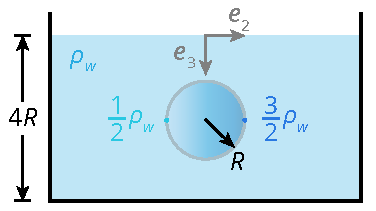
\includegraphics[width=3in]{instr-figures/PS2-Q1.pdf}
\caption{\small{Hydrogel sphere with a linear density gradient submerged in water. The water has a density $\rho_w$, while the sphere has a density at its leftmost point of $\rho_w/2$ and at its rightmost point of $3\rho_w/2$.}}
\end{figure}

\vspace{-1em}
The surface traction $\bm{t}(\bm{x},\hat{\bm{n}})$ acting on $\mathcal{B}$ is given by 
\begin{equation*}
\bm{t}(\bm{x},\hat{\bm{n}}) = -\rho_w g x_3 \hat{\bm{n}},
\end{equation*}
where $\hat{\bm{n}}$ is the outer unit normal to the surface $\partial \Omega_t$ and $\rho_w$ is the (constant) density of water and $g$ is the acceleration due to gravity. 

\medskip
(a) Determine the net force and moment acting on $\mathcal{B}$ via volume integrals.

\medskip
(b) Under what \textit{two} conditions is $\mathcal{B}$ in static equilibrium?


\bigskip
\subsection*{2--3. \textbf{Viscoelastic data} [4 pts].} 
Stress relaxation isochrones for a compliant viscoelastic material are shown in the figure below.  

\begin{figure}[H]
\vspace{-1em}
\centering
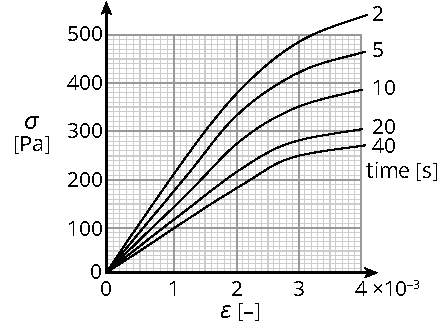
\includegraphics[scale = 1.5]{instr-figures/PS2-Q3.pdf}
\caption{\small{Stress (Pa) vs. strain ($-$) for a soft viscoelastic material.}}
\end{figure}

\vspace{-1em}
(a) Are these isochrones from a material which we can describe with linear viscoelasticity? If not, why not, and if so, under what approximate regimes would this assumption be valid? 

\medskip
(b) Estimate the creep relaxation function $J_c$ for stress values of 100 and 250 \textcolor{red}{Pa}. Isochrones are shown at times of 2, 5, 10, 20, and 40 seconds.   
% This is a placeholder for the example problems from the second problem set. 
% You'll replace this file with the one I supply on canvas. 

\bigskip
\subsection*{2--4. \textbf{Impulsive stresses} [4 pts].}

(a) Say that instead of a step load, we apply $\sigma(t) = A \delta(t)$ to an unknown linear viscoelastic material. 
Determine the strain history $\epsilon(t)$, first as a general function of the creep relaxation function $J_c(t)$, and then for a Kelvin-Voigt solid. 

(b) Now, consider a rapid load followed by a rapid reverse load by applying a doublet function of stress, i.e. $\sigma(t) = B \psi(t)$. 
What is the strain function $\epsilon(t)$ in terms of $J_c(t)$ and for a Kelvin-Voigt material now? 


\bigskip
\subsection*{2--5. \textbf{Two-element models} [8 pts].}

Dynamic mechanical analysis (DMA) is a common technique for characterizing viscoelasticity. 
DMA conventionally involves application of a sinusoidal displacement to the top surface of a sample at a controllable temperature. 
Often, the user puts the sample into initial compression, and follows with the sinusoidal profile. 
A cylindrical sample of height $h$ and diameter $d$ is placed between two plates.
The DMA then quickly puts the sample into compression by moving its top plate downward by a displacement $d$, and then oscillates sinusoidally between positions $0$ and $2d$ at a frequency $\omega$.

\medskip
(a) Using the constitutive law for a Kelvin-Voigt material, determine the stress $\sigma(t)$ exerted by the platens to cause the applied strain. 

\medskip
(b) The resulting stress lags behind the strain by an phase $\delta$, as in $\sin(\omega t + \delta)$. 
Commonly this is reported as the ``tangent loss", or $\tan\delta$, for a material. 
What is the value of $\tan\delta$ for this particular Kelvin-Voigt model?

\medskip
(c) Say instead of prescribing the strain $\epsilon(t)$, we instead prescribed the stress, $\sigma(t) = - \sigma_0 - \sigma_0 \sin(\omega t)$. 
Determine the strain $\epsilon(t)$ for this prescribed stress.

\medskip
(d) Prove that the tangent loss function $\tan\delta$ is identical between the two loading methods.







\section*{Examples I. Mathematical Preliminaries (due \textcolor{red}{Sept 19})}
\textcolor{red}{(Rev note: v2)}
\label{PS1}

This set of example problems is due on September 17, 2025. 
I request that you type up your responses in \LaTeX~ rather than write them out by hand. 
The primary reason is to become better acquainted with writing up mechanics in archival format. 
If you have diagrams, plots, etc., please add them as attached figures using the \texttt{includegraphics} command. 

\bigskip
\subsection*{1--1. \textbf{Convolutional integrals} [4 pts].} The response of a 1D viscoelastic material to an applied forcing function is given using a convolutional integral:
\begin{equation}
    \varepsilon(t) = \int_0^t J(t-\tau) \frac{d\sigma(\tau)}{d\tau} d\tau,
\end{equation}
where $\varepsilon(t)$ is the time-dependent strain response, $\sigma(t)$ is the prescribed stress function, and $J(t)$ is the material compliance, assumed to not depend on the level of stress applied. 
Say we have a compliance function 
\begin{equation}
    J(t) = J_\infty + (J_0-J_\infty)\exp[-t/\tau_c],
\end{equation}
where $J_0, J_\infty, \tau_c$ are all constants $\in \mathbbm{R}$. 
We subject this material to two different loading profiles: (a) step load $\sigma_1(t) = \sigma_0 H(t)$ and (b) a sinusoidal load $\sigma_2(t) = \sigma_0  \sin(\omega t)$, where $\sigma_0$ and $\omega$ are also constant, and $H(t)$ is the step function. 

Determine the corresponding Laplace transforms of the strain functions $\mathcal{L}\{\varepsilon_1(t)\}$ and $\mathcal{L}\{\varepsilon_2(t)\}$. 

\textit{\textbf{Dare mode:}} If you have taken complex analysis, you can compute the inverse transform of polynomial forms because this type of model yields terms with simple poles (i.e. linear in $s$). 
The formulae for this (see e.g. \cite{rileyMathematicalMethodsPhysics2006} Chs. 24 and 25) are:
\begin{equation*}
    \textrm{Residue for simple poles: } R(f(s),s_0) = \lim\limits_{s\rightarrow s_0} \left[ (s-s_0) f(s) \right],
\end{equation*}
and you multiply each residue by the shift from zero, i.e.,
\begin{equation*}
    f(t) = \mathcal{L}^{-1}\{F(s)\} = \sum \left( \textrm{residues of } F(s)e^{s_0 t} \textrm{ at all poles } s_0 \right)
\end{equation*}
\textit{If you dare}, determine the corresponding strain histories $\varepsilon_1(t)$ and $\varepsilon_2(t)$. The first is relatively straightforward; the latter has complex poles and more terms. 

\bigskip
\textit{Solution.}
\begin{align*}
\bm{a.)}\; \mathcal{L}\{\varepsilon_1(t)\} &= \mathcal{L}\{ \int_0^t ( J_\infty + (J_0-J_\infty)\exp[-(t-\tau)/\tau_c]) \frac{d(\sigma_0 H(\tau))}{d\tau} d\tau \} \\
&= \mathcal{L}\{ \int_0^t ( J_\infty + (J_0-J_\infty)\exp[-(t-\tau)/\tau_c]) \sigma_0 \delta(\tau) d\tau \} \\
&= \sigma_0 \mathcal{L}\{ \int_0^t ( J_\infty + (J_0-J_\infty)\exp[-(t-\tau)/\tau_c]) \delta(\tau) d\tau \} \\
&= \sigma_0 \mathcal{L}\{J_\infty + (J_0 - J_\infty)\exp[-t/\tau_c]\} \\
&= \sigma_0 \left(\frac{J_\infty}{s} + \frac{J_0 - J_\infty}{s+\tau^{-1}}\right) \\
\end{align*}
\begin{align*}
\bm{b.)}\; \mathcal{L}\{\varepsilon_2(t)\} &= \mathcal{L}\{ \int_0^t ( J_\infty + (J_0-J_\infty)\exp[-(t-\tau)/\tau_c]) \frac{d(\sigma_0 \sin(\omega \tau))}{d\tau} d\tau \} \\
&= \sigma_0 \omega \mathcal{L}\{ \int_0^t ( J_\infty + (J_0-J_\infty)\exp[-(t-\tau)/\tau_c]) \cos(\omega \tau) d\tau \} \\
&= \sigma_0 \omega \mathcal{L}\{J_\infty + (J_0 - J_\infty)\exp[-t/\tau_c]\} \mathcal{L}\{\cos(\omega t)\} \\
&= \sigma_0 \omega \left( \frac{J_\infty}{s} + \frac{J_0 - J_\infty}{s+\tau_c^{-1}} \right) \frac{s}{s^2+\omega^2}
\end{align*}

I dare not venture further into the land of 501 given time constraints w/ my other work :)
% Recognize the Volterra integral form, which allows the function to be re-written as:


%\newpage
\bigskip
\subsection*{1--2. \textbf{Index notation} [4 pts].} Let $\bm{p}, \bm{q}, \bm{r}, \bm{a}, \bm{b}$ be vector fields on $\mathbbm{R}^3$ and $\bn{Q}$ be a change-of-basis tensor on $\mathbbm{R}^3$. Show the following identities to be true using index notation. 

\begin{itemize}
    \item $\bm{p} \times (\bm{q} \times \bm{r}) = (\bm{r} \cdot \bm{p}) \bm{q} - (\bm{q} \cdot \bm{p}) \bm{r}$
    \item $(\bm{p} \times \bm{q}) \cdot (\bm{a} \times \bm{b}) = (\bm{p} \cdot \bm{a}) (\bm{q} \cdot \bm{b}) - (\bm{q} \cdot \bm{a})(\bm{p} \cdot \bm{b})$
    \item $(\bm{a} \otimes \bm{b})(\bm{p} \otimes \bm{q}) = \bm{a}\otimes\bm{q}(\bm{b} \cdot \bm{p}) $
    \item $\bn{Q}^\intercal\bm{a} \cdot \bn{Q}^\intercal\bm{b} = \bm{a}\cdot\bm{b} $
\end{itemize}

\textit{Solution:}
\begin{align*}
\bm{a.)}\; \text{LHS} &= p_m \bm{e}^{(m)} \times q_i r_j \epsilon_{ijk} \bm{e}^{(k)} \\
 &= p_m q_i r_j \epsilon_{ijk} \epsilon_{mnk} \bm{e}^{(n)} \\
 &= p_m q_i r_j (\delta_{in} \delta_{jm} - \delta_{im} \delta_{jn})\bm{e}^{(n)} \\
 &= (p_j q_n r_j - p_i q_i r_n) \bm{e}^{(n)} \\
 &= r_j p_j q_n \bm{e}^{(n)} - q_i p_i r_n \bm{e}^{(n)} \\ 
 &= (\bm{r} \cdot \bm{p}) \bm{q} - (\bm{q} \cdot \bm{p}) \bm{r} \qed \\
\end{align*}

\begin{align*}
\bm{b.)}\; \text{LHS} &= p_i q_j \epsilon_{ijk} \bm{e}^{(k)} \cdot a_m b_n \epsilon_{mnp} \bm{e}^{(p)} \\
&= p_i q_j a_m b_n \epsilon_{ijk} \epsilon_{mnp} \bm{e}^{(k)} \cdot \bm{e}^{(p)} \\
&= p_i q_j a_m b_n \epsilon_{ijk} \epsilon_{mnp} \delta_{kp} \\
&= p_i q_j a_m b_n \epsilon_{kij} \epsilon_{kmn} \\ 
&= p_i q_j a_m b_n (\delta_{im} \delta_{jn} - \delta_{in} \delta_{jm}) \\
&= p_i q_j a_i b_j - p_i q_j a_j b_i \\
&= (\bm{p} \cdot \bm{a})(\bm{q} \cdot \bm{b}) - (\bm{q} \cdot \bm{a}) (\bm{p} \cdot \bm{b}) \qed \\
\end{align*}

\begin{align*}
\bm{c.)}\; \text{LHS} &= (a_i b_j \bm{e}^{(i)} \otimes \bm{e}^{(j)}) \cdot (p_m q_n \bm{e}^{(m)} \otimes \bm{e}^{(n)}) \\
&= a_i b_j p_m q_n \bm{e}^{(i)} \otimes \bm{e}^{(n)} \delta_{jm} \\
&= a_i \bm{e}^{(i)} \otimes q_n \bm{e}^{(n)} b_jp_j \\
&= \bm{a} \otimes \bm{q} (\bm{b} \cdot \bm{p}) \qed\\
\end{align*}

\begin{align*}
\bm{d.)}\; \text{LHS} &= Q_{ji} a_j^f \bm{e}^{(i)} \cdot Q_{nm} b_n^f \bm{e}^{(m)} \\
&= a_i^e \bm{e}^{(i)} \cdot b_m^e \bm{e}^{(m)} \\
&= a_i^e b_m^e \delta_{im} \\
&= a_i^e b_i^e \\
&= \bm{a} \cdot \bm{b} \qed
\end{align*}

\subsection*{1--3. \textbf{Tensors and vectors} [4 pts].}
The second-order projection tensors $\bn{P}_{\bm{n}}^{||}$ and $\bn{P}_{\bm{n}}^{\perp}$ are useful operators that take a vector $\bm{u}$ and map that vector to its part parallel and perpendicular to a vector $\bm{n}$, respectively. 

They are defined via:
\begin{equation*}
    \bm{u}_{||} = (\bm{u} \cdot \bm{n}) \bm{n} = (\bm{n} \otimes \bm{n}) \bm{u} = \bn{P}_{\bm{n}}^{||} \bm{u},
\end{equation*}
\begin{equation*}
    \bm{u}_{\perp} = \bm{u} - \bm{u}_{||} = (\bn{I} - \bm{n} \otimes \bm{n}) \bm{u} = \bn{P}_{\bm{n}}^{\perp} \bm{u}.
\end{equation*}

The projection tensors have properties
\begin{align*}
    \bn{P}_{\bm{n}}^{||} + \bn{P}_{\bm{n}}^{\perp} &= \bn{I} \\
    \left(\bn{P}_{\bm{n}}^{||} \right)^m &= \bn{P}_{\bm{n}}^{||} ~\forall ~m \in \mathbbm{Z}^+\\
    \left(\bn{P}_{\bm{n}}^{\perp} \right)^m &= \bn{P}_{\bm{n}}^{\perp} ~\forall ~m \in \mathbbm{Z}^+\\
    \bn{P}_{\bm{n}}^{||} \bn{P}_{\bm{n}}^{\perp} = \bn{P}_{\bm{n}}^{\perp} \bn{P}_{\bm{n}}^{||}  &= \bn{0}
\end{align*}

Using the projection tensors, show that $\bm{u} = (\bm{u} \cdot \bm{n}) \bm{n} + \bm{n} \times (\bm{u} \times \bm{n} )$.

\bigskip
\textit{Solution:} \\
From the provided relationship we see that: \\
\begin{align*}
\bm{u} &= \bm{u}_{||} + \bm{u}_{\perp} \\
&= (\bm{u} \cdot \bm{n}) \bm{n} + \bm{u}_{\perp} \\
\end{align*}
Therefore the proof is satisfied if we show that: 
\begin{equation*}
\bm{u}_{\perp} = \bm{n} \times (\bm{u} \times \bm{n})
\end{equation*}

Thus: 
\begin{align*}
\bm{n} \times (\bm{u} \times \bm{n}) &= n_p \bm{e}^{p} \times (u_i n_j \epsilon_{ijk} \bm{e}^{(k)}) \\
&= n_p u_i n_j \epsilon_{pkq} \epsilon_{ijk} \bm{e}^{(q)} \\
&= n_p u_i n_j \epsilon_{qpk} \epsilon_{ijk} \bm{e}^{(q)} \\
&= n_p u_i n_j (\delta_{qi} \delta_{pj} - \delta{qj} \delta_{pi}) \bm{e}^{(q)} \\
&= (n_j u_q n_j - n_i u_i n_q) \bm{e}^{(q)} \\
&= \bm{u} (\bm{n} \cdot \bm{n}) - (\bm{n} \otimes \bm{n}) \bm{u} \\
&= \bm{u} - (\bm{n} \otimes \bm{n}) \bm{u} \\
&= (\bn{I} - \bm{n} \otimes \bm{n}) \bm{u} \\
&= \bm{u}_{\perp} \qed \\
\end{align*}

\bigskip
\subsection*{1--4. \textbf{Vector and tensor calculus} [4 pts].} Show the following vector and tensor identities to be true using index notation:

\begin{itemize}
    \item $\gradX \times (\phi \bm{a}) = \phi \gradX \times \bm{a} + (\gradX\phi) \times \bm{a}$
    \item $\gradX (\bm{a} \cdot \bm{b}) = (\bm{a} \cdot \gradX) \bm{b} + (\bm{b} \cdot \gradX) \bm{a} + \bm{a} \times (\gradX \times \bm{b}) + \bm{b} \times (\gradX \times \bm{a})$
    \item $ (\bn{A} \bn{B}) \bn{:} \bn{C} = (\bn{A}^\intercal \bn{C})\bn{:} \bn{B} = (\bn{C} \bn{B}^\intercal)\bn{:} \bn{A}$
    \item Let $J = \det \bn{F}$. Show\footnote{It will help to use the expression for the determinant of a tensor in index notation!} that $\frac{\partial J}{\partial \bn{F}} = J \bn{F}^{-\intercal}$. 
\end{itemize}

\bigskip
\textit{Solution.}
\begin{align*}
\bm{a.)}\; \text{LHS} &= \epsilon_{ijk}\frac{\partial(\phi a_k)}{\partial x_j} \bm{e}^{(i)} \\
&= \epsilon_{ijk} \left(\frac{\partial \phi}{\partial x_j}a_k + \phi \frac{\partial a_k}{\partial x_j}\right) \bm{e}^{(i)} \\
&= \frac{\partial \phi}{\partial x_j} a_k \epsilon_{jki} \bm{e}^{(i)} + \phi \frac{\partial a_k}{\partial x_j} \epsilon_{jki} \bm{e}^{(i)} \\
&= \nabla_{\bm{X}}\phi \times \bm{a} + \phi \nabla_{\bm{X}} \times \bm{a} \qed \\
\end{align*}

\begin{align*}
\bm{b.)}\; \text{LHS} &= \frac{\partial a_j}{\partial x_i} \mathbf{e}^{(j)} \otimes \mathbf{e}^{(i)} \cdot b_k \mathbf{e}^{(k)} + a_j \mathbf{e}^{(j)} \cdot \frac{\partial b_k}{x_i}\mathbf{e}^{(k)} \otimes \mathbf{e}^{(i)} \\
&= \frac{\partial a_j}{\partial x_i} b_k \mathbf{e}^{(i)} \delta_{jk} + a_j \frac{\partial b_k}{\partial x_i} \delta_{jk} \mathbf{e}^{(i)} \\
&= \frac{\partial a_j}{\partial x_i} b_j \mathbf{e}^{(i)} + a_j \frac{\partial b_j}{\partial x_i} \mathbf{e}^{(i)} \\
&= a_{j,i} b_j \mathbf{e}^{(i)} + b_{j,i} a_j \mathbf{e}^{(i)} \\
\text{RHS} &= a_i b_{j,i} \mathbf{e}^{(j)}  + b_i a_{j,i} \mathbf{e}^{(j)} + a_m \mathbf{e}^{(m)} \times (\epsilon_{ijk} b_{k,j} \mathbf{e}^{(i)}) + b_m \mathbf{e}^{(m)} \times (\epsilon_{ijk} a_{k,j} \mathbf{e}^{(i)}) \\
&= a_i b_{j,i} \mathbf{e}^{(j)}  + b_i a_{j,i} \mathbf{e}^{(j)} + a_m b_{k,j} \epsilon_{ijk} \epsilon_{mip} \mathbf{e}^{(p)}) + b_m a_{k,j} \epsilon_{ijk} \epsilon_{mip} \mathbf{e}^{(p)} \\
&= a_i b_{j,i} \mathbf{e}^{(j)}  + b_i a_{j,i} \mathbf{e}^{(j)} + a_m b_{k,j} \epsilon_{ijk} \epsilon_{ipm} \mathbf{e}^{(p)}) + b_m a_{k,j} \epsilon_{ijk} \epsilon_{ipm} \mathbf{e}^{(p)} \\
&= a_i b_{j,i} \mathbf{e}^{(j)}  + b_i a_{j,i} \mathbf{e}^{(j)} + a_m b_{k,j} (\delta_{jp}\delta_{km} - \delta_{jm}\delta_{kp}) \mathbf{e}^{(p)} + b_m a_{k,j} (\delta_{jp}\delta_{km} - \delta_{jm}\delta_{kp}) \mathbf{e}^{(p)} \\
&= a_i b_{j,i} \mathbf{e}^{(j)}  + b_i a_{j,i} \mathbf{e}^{(j)} + a_k b_{k,j} \mathbf{e}^{(j)} - a_j b_{k,j} \mathbf{e}^{(k)} + b_k a_{k,j} \mathbf{e}^{(j)} - b_j a_{k,j} \mathbf{e}^{(k)} \\
&= a_i b_{j,i} \mathbf{e}^{(j)}  + b_i a_{j,i} \mathbf{e}^{(j)} + a_k b_{k,j} \mathbf{e}^{(j)} - a_i b_{j,i} \mathbf{e}^{(j)} + b_k a_{k,j} \mathbf{e}^{(j)} - b_i a_{j,i} \mathbf{e}^{(j)} \\
&= a_k b_{k,j} \mathbf{e}^{(j)} + b_k a_{k,j} \mathbf{e}^{(j)} \\
&= a_{k,j} b_k \mathbf{e}^{(j)} + b_{k,j} a_k \mathbf{e}^{(j)} \\
&= a_{j,i} b_j \mathbf{e}^{(i)} + b_{j,i} a_j \mathbf{e}^{(i)} \\
\text{LHS} &= \text{RHS} \qed \\
\end{align*}

\begin{align*}
\bm{c.)}\; \text{Term 1} &= (A_{ij} B_{jk} \bm{e}^{(i)} \otimes \bm{e}^{(k)}):(C_{mn} \bm{e}^{(m)} \otimes \bm{e}^{(n)})\\ 
&= A_{ij} B_{jk} C_{mn} \delta_{im} \delta_{kn} \\ 
&= A_{ij} B_{jk} C_{ik} \\ 
\text{Term 2} &= (A_{ji} C_{jk} \bm{e}^{(i)} \otimes \bm{e}^{(k)}) : (B_{mn} \bm{e}^{(m)}  \otimes \bm{e}^{(n)}) \\
&=A_{ji} C_{jk} B_{mn} \delta_{im} \delta_{kn} \\
&= A_{ji} C_{jk} B_{ik} \\
&= A_{ij} B_{jk} C_{ik} \\
\text{Term 3} &= C_{ij} B_{kj} \bm{e}^{(i)} \otimes \bm{e}^{(k)}) : (A_{mn} \bm{e}^{(m)} \otimes \bm{e}^{(n)}) \\
&= C_{ij} B_{kj} A_{mn} \delta_{im} \delta_{kn} \\
&= C_{ij} B_{kj} A_{ik} \\
&= A_{ik} B_{kj} C_{ij} \\
&= A_{ij} B_{jk} C_{ik} \qed \\
\end{align*}

\begin{align*}
\bm{d.)}\; \frac{\partial J}{\partial \bm{F}_{mn}} &= \frac{\partial (\det (\bn{F}))}{\partial \bm{F}_{mn}} \\
&= \frac{\frac{1}{6} \epsilon_{ijk} \epsilon_{pqr} \bn{F}_{ip} \bn{F}_{jq} \bn{F}_{kr}}{\partial \bn{F}_{mn}} \\
&= \frac{1}{6} \epsilon_{ijk} \epsilon_{pqr} \left( \frac{\partial \bn{F}_{ip} \bn{F}_{jq}}{\bn{F}_{mn}} \bn{F}_{kr} + \bn{F}_{ip} \bn{F}_{jq} \frac{\bn{F}_{kr}}{\bn{F}_{mn}} \right) \\
&= \frac{1}{6} \epsilon_{ijk} \epsilon_{pqr} \left( (\delta_{im} \delta_{pn} \bn{F}_{jq} + \bn{F}_{ip} \delta_{jm} \delta_{qn}) \bn{F}_{kr} + \bn{F}_{ip} \bn{F}_{jq} \delta_{km} \delta_{rn} \right) \\
&= \frac{1}{6} (\epsilon_{mjk} \epsilon_{nqr} \bn{F}_{jq} \bn{F}_{kr} + \epsilon_{imk} \epsilon_{pnr} \bn{F}_{ip} \bn{F}_{kr} + \bn{F}_{ip} \bn{F}_{jq} \epsilon_{ijm} \epsilon_{pqn}) \\
&= \frac{1}{6} (\epsilon_{jkm} \epsilon_{qrn} \bn{F}_{jq} \bn{F}_{kr} + \epsilon_{kim} \epsilon_{rpn} \bn{F}_{kr} \bn{F}_{ip} + \epsilon_{ijm} \epsilon_{pqn} \bn{F}_{ip} \bn{F}_{jq}) \\
&= \frac{1}{2} \epsilon_{jkm} \epsilon_{qrn} \bn{F}_{jq} \bn{F}_{kr} \\
\intertext{Multiply both sides by $\bm{F}_{mi}$ to help achieve form of J on RHS:} \\
\frac{\partial J}{\partial \bn{F}_{mn}} \bn{F}_{mi} &= \frac{1}{2} \epsilon_{jkm} \epsilon_{qrn} \bn{F}_{jq} \bn{F}_{kr} \bn{F}_{mi} \\
&= \frac{1}{2} \epsilon_{jkm} \epsilon_{qrn} \bn{F}_{jq} \bn{F}_{kr} \bn{F}_{mn} \delta_{in} \\
&= 3 J \delta_{in}
\intertext{Multiply both sides by $\bm{F}^{-1}_{im}$ to isolate $\frac{\partial J}{\partial \bn{F}}$ term:} \\
(\bn{F}^{-1})_{im} \frac{\partial J}{\partial \bn{F}_{mn}} \bn{F}_{mi} &= 3 J (\bn{F}^{-1})_{im} \delta_{in} \\
\frac{\partial J}{\partial \bn{F}_{mn}} \delta_{ii} &= 3 J (\bn{F}^{-1})_{nm} \\
3 \frac{\partial J}{\partial \bn{F}_{mn}} &= 3 J (\bn{F}^{-T})_{mn} \\
\frac{\partial J}{\partial \bn{F}_{mn}} &= J (\bn{F}^{-T})_{mn} \qed \\
\end{align*}



%\newpage
\bigskip
\subsection*{1--5. \textbf{Kinematics} [8 pts].} The Happy Gelatinous Cube (HGC, pictued) $\mathcal{G}$ exists on a domain of $\{-1\leq X_1 , X_3\leq1, 0\leq X_2 \leq 2\}$ at initial time $t=0$. 
At all times, the bottom surface of the HGC does not move. 
Its top surface moves sinusoidally in time at frequency $\omega$ by a maximum magnitude of $\alpha$. 
At maximum compression, points in the centers of the surfaces defined by outward normals $\bm{e}_1$ and $\bm{e}_3$ experience maximum displacements of magnitude $\beta$. 

\medskip
(a) Determine the deformation gradient tensor $[\bn{F}(\bm{X})]^{\bm{e}}$ for all $\bm{X}\in \mathcal{G}$. 
Describe any assumptions you make about the shape of the HGC as it deforms. 

\medskip
(b) Determine the stretch magnitude of a small fiber positioned at a height $X_2 = 1$ and oriented at an angle $\theta$ from the $\bm{e}_1$ axis \textcolor{red}{(in either the $\bm{e}_1- \bm{e}_2$ or $\bm{e}_1- \bm{e}_3$ plane)}. 

\medskip
(c) Determine the Lagrange-Green strain tensor $\bn{E}$ and the material logarithmic strain tensor $\bn{E}_H = \ln (\bn{U})$ for the geometric center $\bm{X}_c$ of the HGC\footnote{Note that the log of a tensor is defined by writing it spectrally and replacing each eigenvalue with the log of that eigenvalue. For a case of no shear/off-diagonal terms, you can just take the log of each element on the diagonal to get $\ln(\bn{U})$.}. 
What are the maximum and minimum values of the strain eigenvalues $E_i(t)$ and $E_i^H(t)$? 
Would you expect one set to be more symmetric about zero as $\alpha$ gets large, and why?

\medskip
(d) Determine both the material point acceleration $\bm{A}(\bm{X}_1)$ at \textcolor{red}{\sout{, and spatial acceleration $\bm{a}(\bm{x}_1)$ of material moving through,}} a point $\frac{1}{2} \bm{e}_1 + 2\bm{e}_2 + \frac{1}{2} \bm{e}_3$.  

\begin{figure}
\centering
\animategraphics[loop,autoplay,width=4in]{10}{instr-figures/The_Happy_Gelatinous_Cube-}{1}{10}
\end{figure}

\textit{Solution.}

\textbf{a.)} I begin by defining a mapping function $\mathbf{\chi}$:

\begin{equation*}
\mathbf{\chi}(\mathbf{X},t) = \mathbf{X} + \mathbf{u}(\mathbf{X},t) = \begin{bmatrix} X_1 \\ X_2 \\ X_3 \end{bmatrix} + 
\begin{bmatrix}
\beta \sin(\omega t) (1-(1-X_2)^2)X_1 \\
\alpha \sin(\omega t) \frac{X_2}{2} \\
\beta \sin(\omega t) (1-(1-X_2)^2)X_3
\end{bmatrix}
\end{equation*}

This mapping meets all the necessary boundary conditions specified in the problem: (1) $u_2(X_2 = 2) = \sin(\omega t)$, $|u_1(X_2 = 1, X_1 = \pm 1)| = \beta$, and similarly $|u_3(X_2 = 1, X_3 = \pm 1)| = \beta$. It follows that the deformation gradient tensor can be calculated as: 

\begin{align*}
\bn{F}(\mathbf{X},t) &= \nabla_{\mathbf{X}}\mathbf{\chi}(\mathbf{X},t) \\
&= \begin{bmatrix}
    1+\beta \sin(\omega t)(1-(1-X_2)^2 & 2\beta\sin(\omega t)X_1(1-X_2) & 0 \\
    0 & 1 + \frac{\alpha}{2} \sin(\omega t) & 0 \\
    0 & 2\beta\sin(\omega t)X_3(1-X_2) & 1+\beta\sin(\omega t)(1-(1-X_2)^2)
\end{bmatrix}
\end{align*}

\textbf{a.)}

\begin{equation*}
    \bn{F}(X_2 = 1) = \begin{bmatrix}
        1+\beta\sin(\omega t) & 0 & 0 \\ 
        0 & 1 + \frac{\alpha}{2}\sin(\omega t) & 0 \\
        0 & 0 & 1 + \beta \sin(\omega t)
    \end{bmatrix}
\end{equation*}

\textbf{b.)}
\begin{align*}
    \bn{C}(X_2 = 1) &= \bn{F}^T(X_2 = 1) \bn{F}(X_2 = 1) \\
    &= \begin{bmatrix}
        (1+\beta\sin(\omega t))^2 & 0 & 0 \\ 
        0 & (1 + \frac{\alpha}{2}\sin(\omega t))^2 & 0 \\
        0 & 0 & (1 + \beta \sin(\omega t))^2
    \end{bmatrix}
\end{align*}
I will calculate the stretch in the plane made by $\mathbf{e}^{1}$ and $\mathbf{e}^{3}$. A fiber direction $\mathbf{\hat{n}}$ located in this plane with an angle $\theta$ from the $\mathbf{e}^(1)$ axis is: 
\begin{equation*}
\mathbf{\hat{n}} = \begin{bmatrix} \cos(\theta) & 0 & \sin(\theta) \end{bmatrix}
\end{equation*}
\begin{align*}
\lambda(\mathbf{\hat{n}}) &= \sqrt{\mathbf{\hat{n}} \cdot \mathbf{C} \mathbf{\hat{n}}} \\
&= \sqrt{ \begin{bmatrix} \cos(\theta) \\ 0 \\ \sin(\theta) \end{bmatrix} \cdot \begin{bmatrix}
    (1+\beta\sin(\omega t))^2\cos(\theta) \\ 0 \\ (1 + \beta\sin(\omega t))^2\sin(\theta)
\end{bmatrix}} \\
&= \sqrt{(1+\beta\sin(\omega t))^2(\cos^2(\theta) + \sin^2(\theta))} \\ 
&= \sqrt{(1+\beta\sin(\omega t))^2} \\
&= 1+\beta\sin(\omega t))
\end{align*}
Observe that the result will always be positive because it is not a stretch so no absolute value sign is needed. Also note the stretch in the plane does not depend on $\theta$ which aligns with intuition that the central plane of the cube should be axisymmetric about $\mathbf{e}^{(2)}$. 

\textbf{c.)}
Evaluating for Lagrange-Green and logarithmic strains at the centroid of the cube (i.e., $\mathbf{X_c} = [0,1,0]$):
\begin{align*}
\mathbf{E}(\mathbf{X_c}) &= \frac{1}{2}(\mathbf{C}-\mathbf{I)} \\
&= \frac{1}{2} \left(\begin{bmatrix}
    1+2\beta\sin(\omega t)+\beta^2\sin^2(\omega t) & 0 & 0 \\ 0 & 1+ \alpha\sin(\omega t) + \frac{\alpha^2}{4}\sin^2(\omega t) & 0 \\ 0 & 0 & 1 + 2 \beta \sin(\omega t)+\beta^2\sin^2(\omega t)
\end{bmatrix} - \mathbf{I}\right) \\ 
&= \begin{bmatrix}
    \beta\sin(\omega t)(1+\beta\sin(\omega t)) & 0 & 0 \\ 0 & \frac{\alpha}{2}\sin(\omega t)(1 + \frac{\alpha}{4}\sin(\omega t)) & 0 \\ 0 & 0 & \beta\sin(\omega t)(1+\beta\sin(\omega t))
\end{bmatrix}
\end{align*}
\begin{align*}
\mathbf{E_H} &= \ln(\mathbf{U}) \\
&= \ln(\sqrt{\mathbf{C}}) \\
&= \begin{bmatrix}
    \ln(1+\beta\sin(\omega t)) & 0 & 0 \\ 0 & \ln(1+\frac{\alpha}{2}\sin(\omega t)) & 0 \\ 0 & 0 & 1 + \beta\sin(\omega t)
\end{bmatrix}
\end{align*}

I don't need to calculate the eigen values because with the way I defined the mapping function $\mathbf{\chi}$ my deformation gradient tensor and the strains that came from it were already in it's eigen basis. \\

At $t = \frac{n\pi}{\omega}$ the cube is undeformed and the eigen values all equal 1. Then the cube is under-compression in the $\mathbf{e}^{(2)}$ direction, then the $\mathbf{E}_{1,1}$ and $\mathbf{E}_{3,3}$ are the largest eigen values because they will be in tension. This assumes that the Happy Gelatinuous Cube is of course has properties similar to a gelatin-like material and is not auxetic. The same goes for $\mathbf{E}_H$. When the cube is under tension in the direction $\mathbf{e}^{(2)}$, the $\mathbf{E}_{2,2}$ component is the largest eigen value and the other diagonal components are the smallest. \\

As $\alpha$ gets large so too well the magnitudes of the tensile and compressive strains experienced by the specimen. We should except that the logarithmic strains will remain more symmetric. It is worth noting that although in the limit as $\alpha$ approaches $0$ both strain metrics are equivalent, as $\alpha$ becomes large this is not the case. In fact, for a sufficiently large tensile strain, $\mathbf{E}$ tends to $\infty$ whereas at maximum compression the term would approach a Gree-Lagrange strain of $-0.5$. For logarithmic strain, $\ln(\lambda) = -\ln(\lambda^{-1})$ so the magnitude stays much more symmetric for the various terms for the HGC. If let's compare the strains for a single term if stretch is 10 vs $\frac{1}{10}$. Green-Lagrange strains would be 49.5 and -0.4950, respectively whereas logarithmic strain would be 2.30 and -2.30. 

\textbf{d.)}

\begin{align*}
\mathbf{A}(\mathbf{X},t) &= \frac{\partial^2\mathbf{\chi}}{\partial t^2} \\
&= \frac{\partial}{\partial t} \begin{bmatrix}
    \beta\omega\cos(\omega t)(1-(1-X_2)^2)X_1 \\ \alpha\omega\cos(\omega t)\frac{X_2}{2} \\
    \beta\omega\cos(\omega t)(1-(1-X_2)^2)X_3
\end{bmatrix} \\
&= \begin{bmatrix}
    -\beta\omega^2\sin(\omega t)(1-(1-X_2)^2)X_1 \\ -\alpha\omega^2\sin(\omega t)\frac{X_2}{2} \\
    -\beta\omega^2\sin(\omega t)(1-(1-X_2)^2)X_3
\end{bmatrix}
\end{align*}


%% For citations use: 
%%       \citet{<label>} ==> Lamport (1994)
%%       \citep{<label>} ==> (Lamport, 1994)
%%
%Example citation, See \citet{lamport94}.

%% If you have bib database file and want bibtex to generate the
%% bibitems, please use
%%
%%  \bibliographystyle{elsarticle-harv} 
%%  \bibliography{<your bibdatabase>}

%% else use the following coding to input the bibitems directly in the
%% TeX file.

%% Refer following link for more details about bibliography and citations.
%% https://en.wikibooks.org/wiki/LaTeX/Bibliography_Management

%\begin{thebibliography}{00}

%% For authoryear reference style
%% \bibitem[Author(year)]{label}
%% Text of bibliographic item

\bibliographystyle{elsarticle-harv} 
\bibliography{cas-refs}

%\end{thebibliography}
\end{document}

\endinput
%%
%% End of file `elsarticle-template-harv.tex'.


